% =====================================================================
% THIS FILE IS THE SOURCE. Edit it, then rebuild the PDF with:
%     bash tools/compile.sh Unit_04_Prediction_and_Choosing_Predictors
% (run from the Course_Rewrite folder; it compiles twice and reports
%  page count, overfull boxes, and em dashes)
%
% Figures are the fig_u4_*.pdf files in this folder, regenerated by
% tools/make_unit04_slide_figs.py. The data behind them is made up, and
% comes from tools/make_moving_data.py.
% =====================================================================
\documentclass[aspectratio=169]{beamer}
\usetheme{default}
\usefonttheme{professionalfonts}
\usepackage{amsmath, amssymb, amsfonts}
\usepackage{graphicx}
\usepackage{booktabs}
% more air between table rows, they run together otherwise
\renewcommand{\arraystretch}{1.2}
\usepackage{array}
\newcolumntype{L}[1]{>{\raggedright\arraybackslash}p{#1}}
\usepackage{bm}
\usepackage{hyperref}

\mode<presentation> {
    \usetheme{Frankfurt}
    \usecolortheme{default}
}

% == notation shortcuts ==
\newcommand{\xbar}{\bar{x}}
\newcommand{\SE}{\mathrm{SE}}
\newcommand{\se}{\widehat{\SE}}

% Recurring motifs (color-coded).
\newenvironment{principle}[1]{\begin{block}{\textbf{Principle:} #1}}{\end{block}}
\newenvironment{trap}[1]{\begin{alertblock}{\textbf{Trap:} #1}}{\end{alertblock}}
\newenvironment{practice}[1]{\begin{exampleblock}{\textbf{In practice:} #1}}{\end{exampleblock}}
\newenvironment{interview}[1]{\begin{exampleblock}{\textbf{You may be asked:} #1}}{\end{exampleblock}}
\newenvironment{yourturn}[1]{%
  \setbeamercolor{block title}{fg=white,bg=orange!80!black}%
  \setbeamercolor{block body}{bg=orange!12}%
  \begin{block}{\textbf{Your turn:} #1}}{\end{block}}
\newenvironment{livedemo}[1]{%
  \setbeamercolor{block title}{fg=white,bg=teal!80!black}%
  \setbeamercolor{block body}{bg=teal!12}%
  \begin{block}{\textbf{Live demo:} #1}}{\end{block}}
\newenvironment{llmcheck}[1]{%
  \setbeamercolor{block title}{fg=white,bg=violet!75!black}%
  \setbeamercolor{block body}{bg=violet!10}%
  \begin{block}{\textbf{LLM check:} #1}}{\end{block}}

\title{Prediction and Choosing Predictors}
\subtitle{Unit 4: Predicting a New Case, Overfitting, and Which Variables to Keep}
\author{Stat 220 \textbar{} Statistics for Data Science}
\date{}

\begin{document}

\begin{frame}
  \titlepage
\end{frame}

% ======================================================================
\section{Why}
% ======================================================================
\begin{frame}{Where we left off}
\begin{itemize}
  \item Unit 3 fitted a model and read one coefficient at a time.
  \item This unit uses the whole model at once, for two jobs: predicting a case you have
        not seen, and deciding which variables belong in the model.
  \item Both come down to one question: how will this model do on data it was not fitted on?
\end{itemize}
\end{frame}

\begin{frame}{What this unit gives you}
\begin{columns}[T]
\begin{column}{0.5\textwidth}
\textbf{Things to know}
\begin{itemize}\small
  \item how to produce a prediction and an honest interval around it
  \item the difference between a confidence interval and a prediction interval
  \item why error measured on your own data is too small
  \item train/test splits and cross-validation
  \item what underfitting and overfitting look like
  \item how to compare candidate sets of predictors
\end{itemize}
\end{column}
\begin{column}{0.5\textwidth}
\textbf{Mistakes to stop making}
\begin{itemize}\small
  \item quoting a prediction with no interval
  \item quoting a confidence interval when someone asked about one case
  \item reporting the fit on the rows you used to fit it
  \item adding predictors because $R^2$ went up
  \item searching many models and reporting the winner as if you had picked it in advance
  \item predicting outside the range of the data
\end{itemize}
\end{column}
\end{columns}
\end{frame}

\begin{frame}{The data for this unit}
\texttt{moving\_jobs.csv}: 600 completed jobs at a moving company.
\begin{center}\small
\begin{tabular}{L{0.30\textwidth} L{0.60\textwidth}}
\toprule
\textbf{Column} & \textbf{What it is} \\
\midrule
\texttt{hours} & crew time on site, the outcome we predict \\
\texttt{volume\_cuft} & how much is being moved \\
\texttt{crew\_size} & movers assigned, 2 to 4 \\
\texttt{stairs\_flights}, \texttt{miles} & flights of stairs, one-way distance \\
\texttt{packing\_service} & 1 if the customer bought packing \\
\texttt{est\_boxes}, \texttt{dispatcher\_rating}, \texttt{weekend}, \texttt{truck\_id} & also recorded \\
\bottomrule
\end{tabular}
\end{center}
\vspace{0.3em}
The company quotes a customer before the job. Quote too low and the crew runs over.
Quote too high and the customer books someone else.
\end{frame}

% ======================================================================
\section{Making a prediction}
% ======================================================================
\begin{frame}{A prediction is the fitted equation, evaluated at a new case}
\[
   \hat{y}_{\text{new}} = b_0 + b_1 x_{1,\text{new}} + \dots + b_k x_{k,\text{new}}
\]
\begin{itemize}
  \item Put the new case's values into the equation you already fitted.
  \item In code that is one line: \texttt{fit.predict(new)}, where \texttt{new} is a data
        frame with the same columns the model was fitted with.
  \item The number that comes back is a \emph{point} prediction. On its own it is not an answer.
\end{itemize}
\end{frame}

\begin{frame}{Example: quoting a job}
A customer has 800 cubic feet, a crew of 3, two flights of stairs, 12 miles, and wants packing.
\begin{center}\small
\begin{tabular}{lr}
\toprule
predicted hours & 12.39 \\
\bottomrule
\end{tabular}
\end{center}
\begin{itemize}
  \item That is the model's best single guess for this job.
  \item The dispatcher's actual question is different: \emph{how long could this job run?}
  \item Two customers with identical numbers do not take identical time. The model knows that,
        and it can tell you how much they vary.
\end{itemize}
\end{frame}

\begin{frame}{Two different questions, two different intervals}
\begin{itemize}
  \item \textbf{Confidence interval for the line.} Where does the average outcome sit, for jobs
        like this one? It shrinks as the sample grows, because it is about an estimate.
  \item \textbf{Prediction interval for one new case.} Where will \emph{this job} land? It adds
        the job-to-job variation that no model removes, so it stays wide no matter how much data
        you collect.
  \item The prediction interval is always the wider of the two, and it contains the confidence
        interval.
\end{itemize}
\begin{principle}{which one to quote}
If the question is about an average, use the confidence interval. If the question is about one
case, use the prediction interval. A dispatcher scheduling one crew is asking about one case.
\end{principle}
\end{frame}

\begin{frame}{The same job, both intervals}
\begin{center}\small
\begin{tabular}{lcc}
\toprule
& \textbf{95\% interval} & \textbf{width} \\
\midrule
confidence interval, average job like this one & 12.25 to 12.54 & 0.3 hours \\
prediction interval, this one job & 10.74 to 14.04 & 3.3 hours \\
\bottomrule
\end{tabular}
\end{center}
\begin{itemize}\small
  \item Same model, same customer, same prediction of 12.39 hours.
  \item The first interval is eleven times narrower. Quoting it to a dispatcher would promise
        a precision the model never had.
\end{itemize}
\begin{trap}{the default output}
Software often prints the narrow one first. Check which interval you are looking at before
it reaches a customer.
\end{trap}
\end{frame}

\begin{frame}{The two intervals, drawn}
\centering
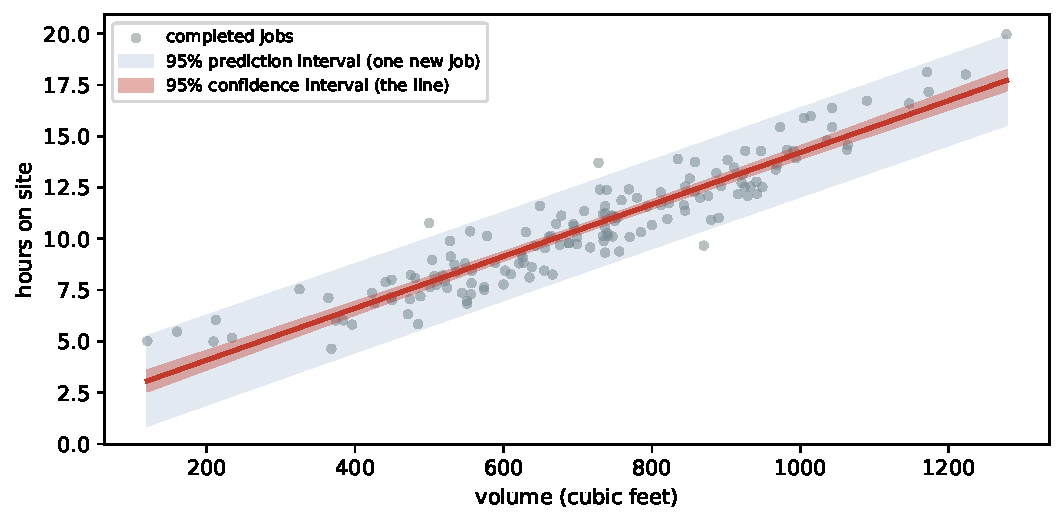
\includegraphics[width=0.84\textwidth]{fig_u4_intervals.pdf}\par
\vspace{0.6em}
\begin{minipage}{0.86\textwidth}\small
The narrow dark band is the \textbf{confidence interval} for the line. The wide pale band is
the \textbf{prediction interval} for a single new job, and about 95\% of the completed jobs
fall inside it.
\end{minipage}
\end{frame}

\begin{frame}{Your turn \#1}
\begin{yourturn}{which interval does each question need?}
\begin{enumerate}
  \item ``If we did a hundred jobs like this one, what would our average time be?''
  \item ``The Thompson move is Tuesday. How many hours should I block on the schedule?''
  \item ``Across all 600 jobs, is packing service associated with longer jobs?''
\end{enumerate}
\vspace{0.2em}
Decide with a neighbor which of the three needs the interval for one new case.
\end{yourturn}
\end{frame}

\begin{frame}{Your turn \#1: answer}
\begin{itemize}
  \item \textbf{(1) Confidence interval.} It asks about an average over many jobs.
  \item \textbf{(2) Prediction interval.} One move, one crew, one Tuesday. This is the wide one,
        and the one people most often get wrong.
  \item \textbf{(3) Neither.} That is a question about a coefficient, which is Unit 3. It asks
        what the model says about a relationship, not what will happen next.
\end{itemize}
\end{frame}

\begin{frame}{Predicting outside the range of the data}
\begin{columns}[c]
\begin{column}{0.58\textwidth}
\centering
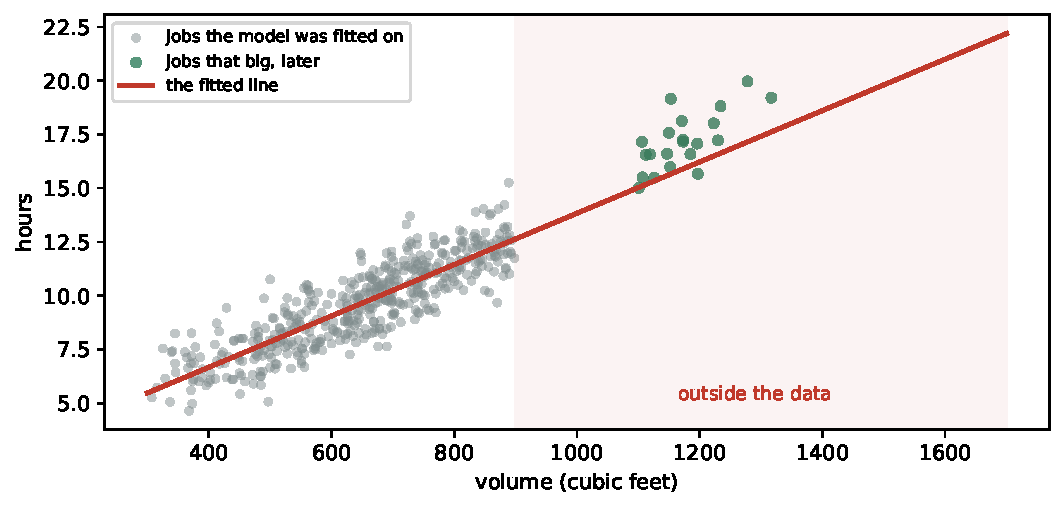
\includegraphics[width=\textwidth]{fig_u4_extrap.pdf}
\end{column}
\begin{column}{0.42\textwidth}
\small
\begin{itemize}
  \item The line was fitted on jobs from 300 to 900 cubic feet.
  \item Asked about a 1,400-cubic-foot job, it answers without complaint.
  \item The jobs that size, when they came in, took longer than the line said. Nothing in the
        fitted data could have told you that.
\end{itemize}
\end{column}
\end{columns}
\end{frame}

% ======================================================================
\section{Honest error}
% ======================================================================
\begin{frame}{Error measured on your own data is too small}
\begin{itemize}
  \item The coefficients were chosen to make the residuals small \emph{on those rows}.
  \item So the error you compute on them is not what you will see on a new job. It is the best
        case, not the typical case.
  \item The fix is to measure on rows the model has not seen.
\end{itemize}
\begin{principle}{the only honest number}
Report error on data the model was not fitted on. Every other number is a description of how
well it memorized.
\end{principle}
\end{frame}

\begin{frame}{The same model, both ways}
Five predictors, 600 jobs, 70\% used for fitting and 30\% held back:
\begin{center}\small
\begin{tabular}{lc}
\toprule
& \textbf{typical error} \\
\midrule
on the rows it was fitted on & 0.79 hours \\
on the rows held back & 0.93 hours \\
\bottomrule
\end{tabular}
\end{center}
\begin{itemize}\small
  \item The gap here is modest, because this model is simple and the sample is large.
  \item The gap grows with model flexibility, and it is largest exactly when you are most
        pleased with your fit.
\end{itemize}
\end{frame}

\begin{frame}{Holding rows back}
\begin{itemize}
  \item \textbf{Train/test split.} Fit on most of the rows, measure on the rest.
        \texttt{train\_test\_split(X, y, test\_size=0.3)}.
  \item One split is a single draw, so the number wobbles depending on which rows landed where.
  \item \textbf{Cross-validation} averages over several splits, so every row is held out once.
\end{itemize}
\end{frame}

\begin{frame}{$K$-fold cross-validation}
\centering
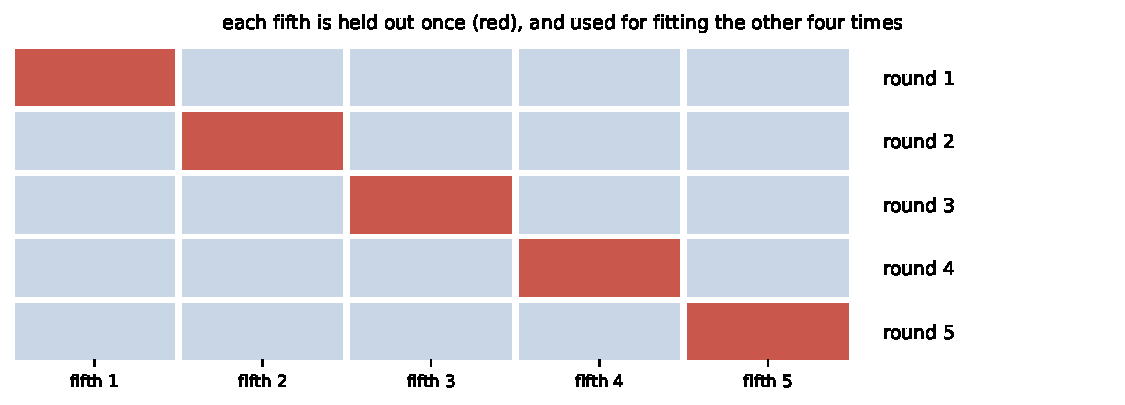
\includegraphics[width=0.82\textwidth]{fig_u4_cv.pdf}
\vspace{0.3em}
\begin{itemize}\small
  \item Split the rows into $K$ pieces, here 5. Fit on four, measure on the fifth, and rotate.
  \item Average the five errors. That average is your estimate of error on a new job.
  \item \texttt{cross\_val\_score(model, X, y, cv=KFold(5, shuffle=True, random\_state=0))}
\end{itemize}
\end{frame}

\begin{frame}{Two ways to get this wrong}
\begin{itemize}
  \item \textbf{Using the held-out rows to choose.} Try twenty models, keep the one with the
        best held-out error, and report that error. It is now a best-of-twenty, which is
        optimistic for the same reason as before.
  \item \textbf{Touching the held-out rows early.} Filling in missing values, scaling, or
        picking predictors using all the data leaks the held-out rows into the fitting.
\end{itemize}
\begin{trap}{the number you report}
Choosing with held-out data is fine. Reporting that same number as your final answer is not.
If the choice mattered, keep a slice you never touched, or say plainly that the number came
from the same data you chose with.
\end{trap}
\end{frame}

% ======================================================================
\section{Too simple, too flexible}
% ======================================================================
\begin{frame}{Two ways a model can be wrong}
\begin{itemize}
  \item \textbf{Underfitting.} The model is too rigid to capture the pattern that is there.
        It is wrong in the same direction for whole stretches of the data.
  \item \textbf{Overfitting.} The model is flexible enough to follow the noise. It fits the
        rows it saw and misses the next ones.
  \item Both show up as large error on new data, which is why you measure there.
\end{itemize}
\end{frame}

\begin{frame}{The same 40 jobs, three models}
\centering
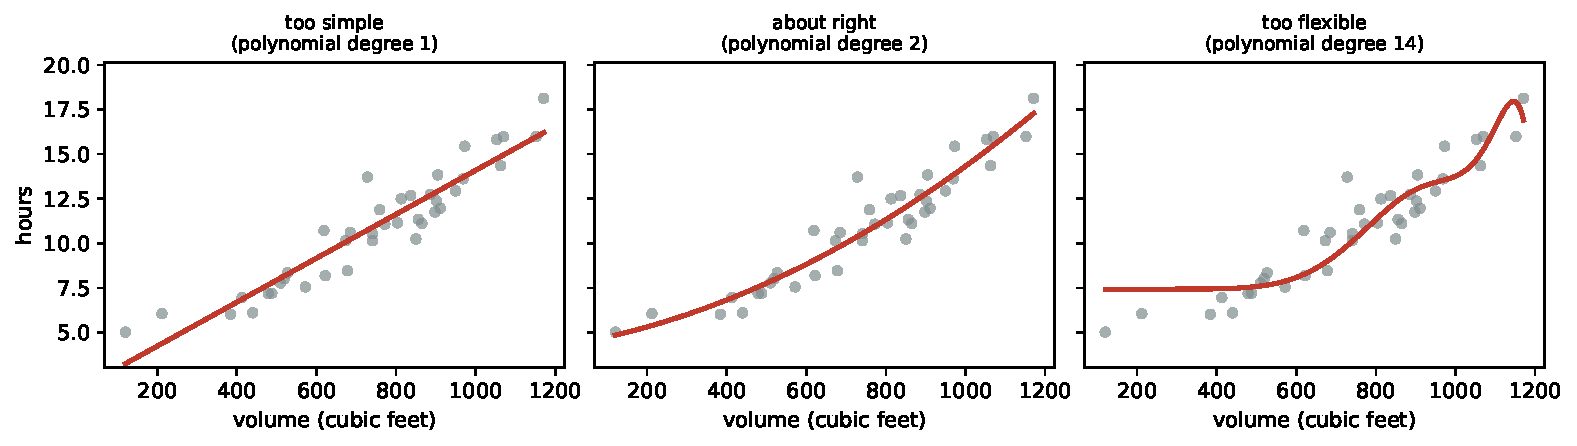
\includegraphics[width=\textwidth]{fig_u4_flex.pdf}\par
\vspace{0.5em}
\begin{minipage}{0.92\textwidth}\small
Left: a straight line misses the bend at the high end. Middle: one curve, about right.
Right: degree 14 passes near almost every point, and the wiggles are noise.
\end{minipage}
\end{frame}

\begin{frame}{Training error and held-out error, as complexity grows}
\begin{columns}[c]
\begin{column}{0.58\textwidth}
\centering
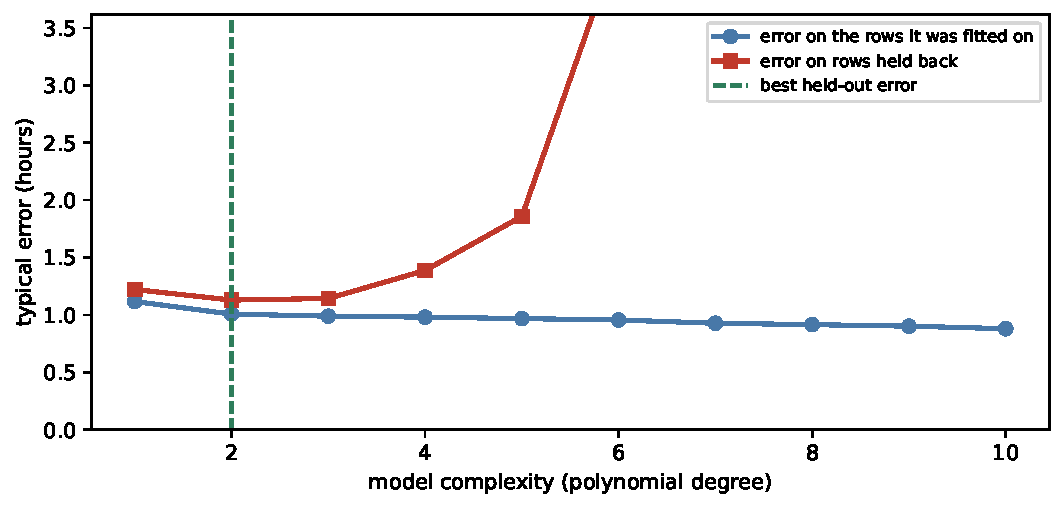
\includegraphics[width=\textwidth]{fig_u4_curve.pdf}
\end{column}
\begin{column}{0.42\textwidth}
\small
\begin{itemize}
  \item Error on the fitted rows falls as you add flexibility, and keeps falling.
  \item Error on held-out rows falls, bottoms out, then climbs. Here it runs off the top of
        the chart.
  \item The bottom of the red curve is the complexity you want.
\end{itemize}
\end{column}
\end{columns}
\end{frame}

\begin{frame}{How much complexity you can afford}
\begin{center}\small
\begin{tabular}{L{0.34\textwidth} L{0.56\textwidth}}
\toprule
\textbf{When this is true} & \textbf{You can support} \\
\midrule
more rows & more flexibility \\
less noise in the outcome & more flexibility \\
a strong, simple relationship & less flexibility, and you do not need more \\
few rows, noisy outcome & a simple model, and honest error bars \\
\bottomrule
\end{tabular}
\end{center}
\vspace{0.3em}
There is no complexity that is right in general. It depends on how much data you have and
how noisy it is, which is why you check rather than guess.
\end{frame}

\begin{frame}{Your turn \#2}
\begin{yourturn}{diagnose the model}
A colleague reports: \textbf{$R^2 = 0.98$ on the data they fitted}, and a typical error of
\textbf{4.1 hours} on jobs from the following month. The model has 60 predictors and was
fitted on 200 jobs.
\vspace{0.2em}

Is this underfitting or overfitting, and what would you change first?
\end{yourturn}
\end{frame}

\begin{frame}{Your turn \#2: answer}
\begin{itemize}
  \item \textbf{Overfitting.} Nearly perfect on its own rows, badly off on new ones, with 60
        predictors for 200 jobs.
  \item \textbf{First change:} cut the model down to the handful of predictors that have a
        reason to be there, then compare by cross-validation.
  \item A useful check: if a model has nearly as many predictors as it has rows, it can fit
        almost anything, including noise.
\end{itemize}
\end{frame}

% ======================================================================
\section{Choosing predictors}
% ======================================================================
\begin{frame}{Adding a predictor never hurts the fit on your own data}
\begin{itemize}
  \item $R^2$ cannot go down when you add a variable. Even a column of random numbers nudges
        it up.
  \item So $R^2$ cannot tell you whether a variable belongs. Neither can ``the coefficient
        came out significant,'' if you went looking through many variables.
  \item You need a criterion that charges you for complexity, or a measurement on data you
        did not fit.
\end{itemize}
\end{frame}

\begin{frame}{Four numbers people use}
\begin{center}\small
\begin{tabular}{L{0.22\textwidth} L{0.70\textwidth}}
\toprule
\textbf{Number} & \textbf{What it does} \\
\midrule
$R^2$ & share of variation explained. Always rises with more predictors, so it cannot choose \\
adjusted $R^2$ & $R^2$ with a small charge per predictor. Better, but a weak guard \\
AIC, BIC & fit with a charge per predictor. Lower is better. BIC charges more, so it picks
smaller models \\
cross-validated error & measured on rows left out. Slower to compute, and closest to the
question you care about \\
\bottomrule
\end{tabular}
\end{center}
\vspace{0.2em}
\small
AIC and BIC compare models fitted to the same rows with the same outcome. Cross-validated
error compares anything that can make a prediction.
\end{frame}

\begin{frame}{Four candidate sets, scored every way}
\begin{center}\footnotesize
\begin{tabular}{lccccc}
\toprule
\textbf{Predictors} & \textbf{$R^2$} & \textbf{adj. $R^2$} & \textbf{AIC} & \textbf{BIC} & \textbf{CV error} \\
\midrule
volume & 0.8717 & 0.8715 & 1766.7 & 1775.5 & 1.056 \\
volume, crew & 0.8873 & 0.8870 & 1690.9 & 1704.1 & 0.991 \\
the five that make sense & 0.9197 & 0.9190 & \textbf{1493.9} & \textbf{1520.2} & 0.840 \\
those five plus three junk columns & \textbf{0.9202} & \textbf{0.9191} & 1496.4 & 1535.9 & \textbf{0.839} \\
\bottomrule
\end{tabular}
\end{center}
\begin{itemize}\small
  \item The junk columns (estimated boxes, dispatcher rating, weekend) raise $R^2$, and even
        nudge adjusted $R^2$ up.
  \item AIC and BIC both get worse. Cross-validated error is a tie, 0.001 hours apart.
  \item Three extra columns bought four seconds of accuracy on a twelve-hour job.
\end{itemize}
\end{frame}

\begin{frame}{The same comparison, drawn}
\centering
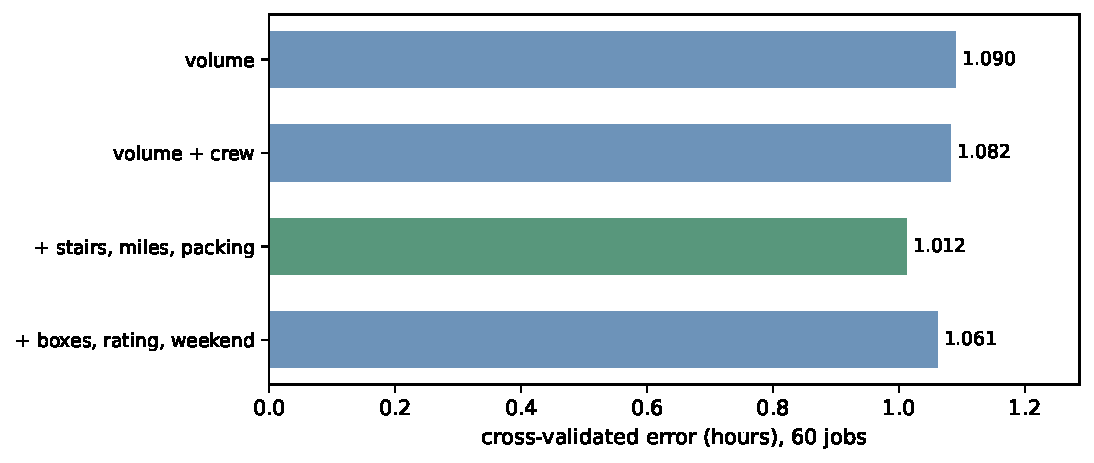
\includegraphics[width=0.78\textwidth]{fig_u4_sets.pdf}
\vspace{0.2em}
\begin{principle}{prefer the simpler model when the scores are close}
A smaller model is easier to explain, cheaper to collect data for, and less exposed to a
column that quietly changes meaning next quarter. Take the extra complexity only when it
buys something you can point at.
\end{principle}
\end{frame}

\begin{frame}{Searching through variables is itself a way to overfit}
\begin{itemize}
  \item Every candidate column gets a chance to look good by luck. With 20 columns that have
        nothing to do with the outcome and a 0.05 cutoff, about one of them clears the bar.
  \item So a variable that survives a long search is not the same as a variable that passed a
        test you planned in advance.
  \item The junk columns in the table above had $p$-values of 0.13, 0.30, and 0.80. That is what
        unrelated columns normally look like. The danger is in what happens when you keep hunting.
\end{itemize}
\end{frame}

\begin{frame}{What stepwise selection does}
\textbf{Stepwise selection} builds the model by repeatedly adding or dropping one variable.
\begin{center}\small
\begin{tabular}{L{0.24\textwidth} L{0.66\textwidth}}
\toprule
\textbf{Version} & \textbf{The loop} \\
\midrule
forward & start with nothing. Add whichever remaining variable helps most. Stop when none helps \\
backward & start with everything. Drop the weakest variable. Stop when dropping hurts \\
both directions & alternate: add the best, then reconsider dropping what is already in \\
\bottomrule
\end{tabular}
\end{center}
\vspace{0.3em}
``Helps most'' is usually the smallest $p$-value, sometimes the biggest drop in AIC. The
procedure runs without your judgment, which is why it is popular and where the trouble
starts.
\end{frame}

\begin{frame}{What that looks like when you run it}
\textbf{Setup.} 50 jobs. The five predictors that make sense, plus 40 columns of pure noise that
we generated ourselves, so we know for a fact they mean nothing. Then forward selection, adding
whatever has the smallest $p$-value, stopping at 0.05.
\begin{center}\small
\begin{tabular}{lc}
\toprule
columns offered & 45 \\
columns kept & 5 \\
of those, pure noise & 1 \\
$p$-value of the noise column in the final model & 0.045 \\
real predictor dropped along the way & \texttt{miles} \\
$R^2$ of the selected model & 0.94 \\
\bottomrule
\end{tabular}
\end{center}
\end{frame}

\begin{frame}{The selected model, as it would be reported}
\centering
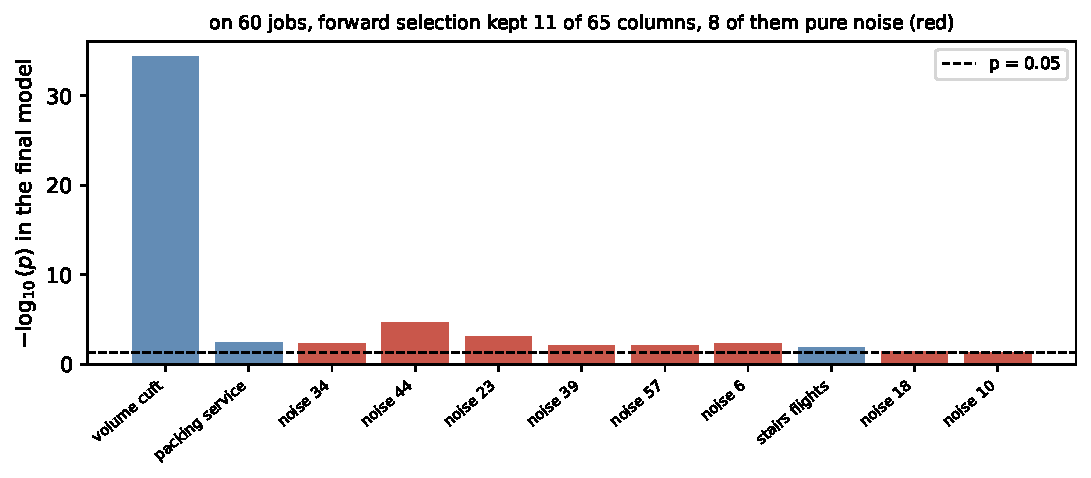
\includegraphics[width=0.74\textwidth]{fig_u4_stepwise.pdf}\par
\vspace{0.4em}
\begin{minipage}{0.88\textwidth}\small
Written up, this model has five predictors, all significant, and an $R^2$ of 0.94. Nothing in
the output says that one of them is a column of random numbers, or that a real predictor was
thrown out to make room for it.
\end{minipage}
\end{frame}

\begin{frame}{Why the $p$-values stop meaning what they say}
\begin{itemize}
  \item A $p$-value answers: if this variable did nothing, how often would a result this strong
        appear? That question assumes you picked the variable \emph{before} looking.
  \item In a search you did not pick it. You picked the best of 45, and the best of 45 is
        extreme by construction.
  \item The same applies to $R^2$ and to the coefficient. All three are reported as if the model
        arrived in one step, when it is the survivor of a tournament.
\end{itemize}
\begin{trap}{what to listen for}
``We started with everything we had and let the procedure decide.'' When you hear that, ask how
many variables went in, and whether the model was checked on data that had no part in choosing it.
\end{trap}
\end{frame}

\begin{frame}{What to do instead, and what to ask}
\begin{columns}[T]
\begin{column}{0.5\textwidth}
\textbf{Instead}
\begin{itemize}\small
  \item write down a few candidate sets, each with a reason, and compare those
  \item judge them on held-out data, where a lucky column gets no credit
  \item let subject knowledge decide the borderline cases
  \item if you do search, do the searching inside the cross-validation, not before it
\end{itemize}
\end{column}
\begin{column}{0.5\textwidth}
\textbf{Ask, of someone else's model}
\begin{itemize}\small
  \item how many variables were considered, not how many are in the model
  \item was the final model checked on data that played no part in choosing it
  \item does each variable have a reason beyond having survived
  \item would the same procedure on last year's data produce the same model
\end{itemize}
\end{column}
\end{columns}
\end{frame}

\begin{frame}{Penalized regression: pay for the size of your coefficients}
\begin{itemize}
  \item Least squares picks coefficients to make the squared residuals as small as possible, and
        nothing stops a coefficient from growing to chase noise.
  \item \textbf{Penalized regression} adds a charge for the size of the coefficients, so a
        variable has to earn its keep against that charge.
\end{itemize}
\[
  \underbrace{\sum (y_i - \hat{y}_i)^2}_{\text{fit the data}}
  \;+\;
  \lambda \underbrace{\sum_j |b_j|}_{\text{charge for size}}
\]
\begin{itemize}
  \item $\lambda$ is the size of the charge. At $\lambda = 0$ you are back to ordinary least
        squares. As $\lambda$ grows, every coefficient is pulled toward zero.
\end{itemize}
\end{frame}

\begin{frame}{Ridge and lasso}
\begin{center}\small
\begin{tabular}{L{0.16\textwidth} L{0.26\textwidth} L{0.46\textwidth}}
\toprule
\textbf{Name} & \textbf{Charge} & \textbf{What it does} \\
\midrule
ridge & $\lambda \sum b_j^2$ & shrinks every coefficient toward zero, but never all the way.
Keeps all the variables \\
lasso & $\lambda \sum |b_j|$ & shrinks, and sends weak coefficients \emph{exactly} to zero,
which drops those variables \\
\bottomrule
\end{tabular}
\end{center}
\begin{itemize}\small
  \item Lasso therefore does selection and fitting in one step, which is why it comes up in a
        unit about choosing predictors.
  \item Ridge is the better choice when predictors are highly correlated and you want to keep
        them all, sharing the credit rather than picking one.
  \item Both need the predictors on a common scale first, because the charge is on the size of
        the coefficient, and a coefficient's size depends on its units.
\end{itemize}
\end{frame}

\begin{frame}{Why a worse fit on your own data can be a better model}
\begin{itemize}
  \item Shrinking always makes the fit on your own rows worse.
  \item In exchange, the coefficients move around less from sample to sample, so the model does
        better on the next job.
  \item It is the complexity curve again, with $\lambda$ as the dial: too little penalty
        overfits, too much underfits, and the best value is somewhere in between.
\end{itemize}
\begin{principle}{what the penalty buys}
A penalty gives up accuracy on the data you have, for accuracy on the data you do not have yet.
\end{principle}
\end{frame}

\begin{frame}{Choosing $\lambda$, and watching the coefficients shrink}
\centering
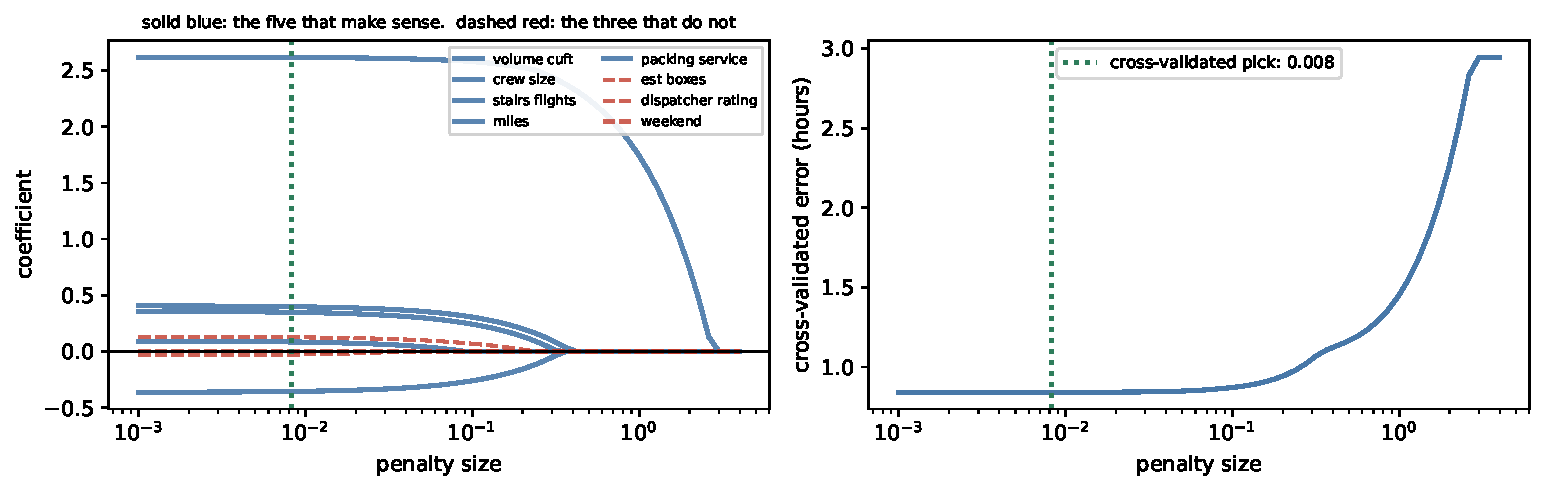
\includegraphics[width=0.94\textwidth]{fig_u4_lasso.pdf}\par
\vspace{0.4em}
\begin{minipage}{0.94\textwidth}\small
Left: each line is one coefficient as the penalty grows. Right: cross-validated error for each
penalty, which is how $\lambda$ gets chosen. The dotted line is the chosen value in both panels.
\end{minipage}
\end{frame}

\begin{frame}{What lasso did with the moving data}
\begin{center}\small
\begin{tabular}{lcl}
\toprule
\textbf{Column} & \textbf{Coefficient} & \textbf{} \\
\midrule
volume & 2.62 & the main driver, barely shrunk \\
packing service & 0.40 & kept \\
stairs & 0.35 & kept \\
crew size & $-0.36$ & kept \\
miles & 0.09 & kept, small \\
estimated boxes & 0.13 & kept, and it is mostly a copy of volume \\
dispatcher rating & $-0.03$ & shrunk to almost nothing \\
weekend & 0.00 & sent to exactly zero, and dropped \\
\bottomrule
\end{tabular}
\end{center}
\vspace{0.2em}
\small
It dropped one of the three junk columns outright and crushed a second. It kept estimated boxes,
which duplicates volume, so the two of them split the credit between them.
\end{frame}

\begin{frame}{What a penalized coefficient is not}
\begin{itemize}
  \item \textbf{It is not an unbiased estimate.} It was deliberately pulled toward zero, so
        reading it as the effect of that variable understates it.
  \item \textbf{A zero is not proof of no relationship.} It means the variable did not earn its
        keep against the penalty, in this sample, alongside these other variables.
  \item \textbf{Being kept is not proof of importance either}, especially when two predictors
        carry nearly the same information and the choice between them is close to a coin flip.
\end{itemize}
\begin{practice}{how to say it}
``Lasso with the penalty chosen by cross-validation kept these six variables. I am using it to
predict, not to claim which variables matter.''
\end{practice}
\end{frame}

\begin{frame}{A recipe you can defend}
\begin{enumerate}
  \item \textbf{Start from the question.} Predicting, or explaining a particular effect?
        The answer changes which variables must be in the model.
  \item \textbf{Write down a small number of candidate sets}, each with a reason. Three or
        four, not every subset.
  \item \textbf{Score them the same way}, with cross-validated error, or AIC and BIC if the
        models are comparable.
  \item \textbf{Take the simplest set that is close to the best.}
  \item \textbf{Report how you chose}, including the sets that lost.
\end{enumerate}
\end{frame}

\begin{frame}{Your turn \#3}
\begin{yourturn}{is the new column worth keeping?}
The company starts recording \textbf{elevator (yes/no)}. Adding it moves $R^2$ from 0.9197 to
0.9206, AIC from 1493.9 to 1492.1, and cross-validated error from 0.840 to 0.835.
\vspace{0.2em}

Keep it or not? What would you want to know before deciding?
\end{yourturn}
\end{frame}

\begin{frame}{Your turn \#3: answer}
\begin{itemize}
  \item Every number moved the right way, and unlike the junk columns, AIC improved rather
        than got worse. That is mild evidence the column carries real information.
  \item The gain is 0.005 hours, about 20 seconds. The case for keeping it is that stairs and
        elevators plainly affect a move, not that the numbers jumped.
  \item Worth knowing: is it recorded for every job, and is it recorded \emph{before} the
        quote? A predictor you will not have at prediction time is useless, however well it
        scores.
\end{itemize}
\end{frame}

% ======================================================================
\section{LLM check}
% ======================================================================
\begin{frame}{LLM check: mistake or not? (1 of 2)}
\begin{llmcheck}{we asked an LLM to evaluate a model}
\textbf{We told it:} ``I fitted a model on all 600 jobs and the $R^2$ is 0.94. Is it good
enough to quote customers with?''\\[4pt]
\textbf{It answered:} ``An $R^2$ of 0.94 means the model explains 94\% of the variation, so it
is performing very well and is suitable for quoting.''
\end{llmcheck}
\vspace{0.2em}
\centering\small Mistake, or no mistake? Decide before we click.
\onslide<2->{%
\begin{trap}{verdict: mistake}
The 0.94 was measured on the rows the model was fitted on, and quoting is a question about one
new job. The right answer is a cross-validated error and a prediction interval.
\end{trap}}
\end{frame}

\begin{frame}{LLM check: mistake or not? (2 of 2)}
\begin{llmcheck}{same data, a different answer}
\textbf{We told it:} ``Adding three more columns raised $R^2$ from 0.9197 to 0.9202. Should I
keep them?''\\[4pt]
\textbf{It answered:} ``That rise is what $R^2$ does when you add any column. Check a criterion
that charges for complexity, such as AIC, or compare cross-validated error, and keep the
columns only if they earn it.''
\end{llmcheck}
\vspace{0.2em}
\centering\small Mistake, or no mistake?
\onslide<2->{%
\begin{principle}{verdict: no mistake}
This is the right move, and it names the reason: $R^2$ rises mechanically, so it cannot be
the deciding number.
\end{principle}}
\end{frame}

% ======================================================================
\section{Consolidate}
% ======================================================================
\begin{frame}{Producing a prediction you can defend}
\small
\begin{enumerate}
  \item \textbf{Fit the model} on the data you have.
  \item \textbf{Check the range.} Is the new case inside the data the model was fitted on?
  \item \textbf{Predict:} \texttt{fit.predict(new)}, with the same columns as the fit.
  \item \textbf{Decide which interval} the question needs: confidence, or prediction.
  \item \textbf{Measure error honestly}, on held-out rows or by cross-validation.
  \item \textbf{Report the number with its interval}, and say what it is an interval for.
\end{enumerate}
\end{frame}

\begin{frame}{The traps, all in one place}
\begin{trap}{the ones that bite most often}
\begin{itemize}
  \item Reporting a prediction with no interval.
  \item Quoting a confidence interval when the question was about one case.
  \item Reporting $R^2$ or error from the rows the model was fitted on.
  \item Adding predictors because $R^2$ rose.
  \item Running a long search and reporting the winner's $p$-value as if it were planned.
  \item Choosing a model on held-out data and reporting that same error as the final number.
  \item Predicting outside the range of the data.
  \item Keeping a predictor you will not have when the prediction is actually needed.
\end{itemize}
\end{trap}
\end{frame}

\begin{frame}{What you should be able to do with software}
\small
You are not expected to memorize syntax. You are expected to know which procedure the question
calls for, what to hand it, and what the output means.
\begin{center}\footnotesize
\begin{tabular}{p{0.44\textwidth} p{0.46\textwidth}}
\toprule
\textbf{You should be able to} & \textbf{What you would reach for} \\
\midrule
Predict a new case & \texttt{fit.predict(new\_df)} \\
Both intervals at once & \texttt{fit.get\_prediction(new\_df)} \newline
\texttt{\phantom{xx}.summary\_frame()} \\
Hold rows back & \texttt{train\_test\_split(X, y, test\_size=0.3)} \\
Cross-validate & \texttt{cross\_val\_score(model, X, y,} \newline
\texttt{\phantom{xx}cv=KFold(5, shuffle=True))} \\
Compare models by AIC or BIC & \texttt{fit.aic}, \texttt{fit.bic} \\
Penalized regression & \texttt{LassoCV(cv=5).fit(X\_scaled, y)} \\
\bottomrule
\end{tabular}
\end{center}
\end{frame}

\begin{frame}{Where we go next}
\begin{itemize}
  \item This unit asked how a model behaves on data it has not seen, and which variables
        deserve to be in it.
  \item Unit 5 asks a different question: where the data came from in the first place, and
        when a coefficient can be read as an effect rather than an association.
  \item A model can predict well and still be the wrong basis for a decision about what to
        change. That distinction is the next unit.
\end{itemize}
\end{frame}

\end{document}
